\documentclass{article}	% essential first line
\usepackage{float}		% this is to place figures where requested!
\usepackage{times}		% this uses fonts which will look nice in PDF format
\usepackage{graphicx}		% needed for the figures
\usepackage{url}
\usepackage{sbc-template} 
\usepackage[scaled]{uarial}


%% Here I adjust the margins

\oddsidemargin 0.1in		% Left margin is 1in + this value
\textwidth 6.25in		% Right margin is not set explicitly
\topmargin -0.2in			% Top margin is 1in + this value
\textheight 9in			% Bottom margin is not set explicitly
\columnsep 0.25in		% separation between columns

%% Define a macro for inserting postscript images
%% ==============================================
%% This is a macro which nominally takes 3 parameters, 
%% it would be used as follows to insert and encapsulated postscript
%% image at the location where it is used.
%%
%% \EPSFIG{epsfilename}{caption}{label}
%% - epsfilename is the name of the encapsulated postscript file to be
%%               inserted at this location
%% - caption is the text to be shown as the figure caption, it will be
%%           prepended by Figure X.  The number X can be referenced
%%           using the label parameter.
%% - label is a name given to the figure, it can be referenced using the
%%         \ref{label} command.

\def\EPSFIG[#1]#2#3#4{		% Don't be scared by this monsrosityok
\begin{figure}[H]		% it is a macro to save typing later
\begin{center}			% 
\includegraphics[#1]{#2}	%
\end{center}			%
\caption{#3}			%
\label{#4}			%
\end{figure}			%
}				%


%% Define the fields to be displayed by a \maketitle command\includegraphics[]{tech_report_vv.pdf}

\sloppy
\author{Felipe M. Besson \\ Pedro M. B. Leal}
\title{\begin{huge}\textbf{User Guide}\end{huge} \\ Baile V\&V Prototype}
 
\address{Department of Computer Science \\ Institute of Mathematics and Statistics\\
University of S\~ao Paulo (USP) 
\email{\{besson,pedrombl\}@ime.usp.br} }


\begin{document}	% Critical
\maketitle			% Use the \author, \title and \date info

\date 


\newpage

\section{ Prerequisites}
The following software elements must be installed and working:

\begin{itemize}
 \item Java 6~\cite{java6}
 \item SQLite 3~\cite{sql3}
 \item Ant~\cite{ant}
\end{itemize}

\section{ Where to download ? }
The source code, the scripts and its dependecies are available on:

\section{ How to use ? }
In this section, we detailed the main steps to interact with the application.

\begin{enumerate}
 \item Start the script \textbf{baile.sh}, and then, the application will start:

  \begin{figure}[htbp]
  \centering
  \setlength\fboxrule{1.0pt}
  \scalebox{0.5}{\fbox{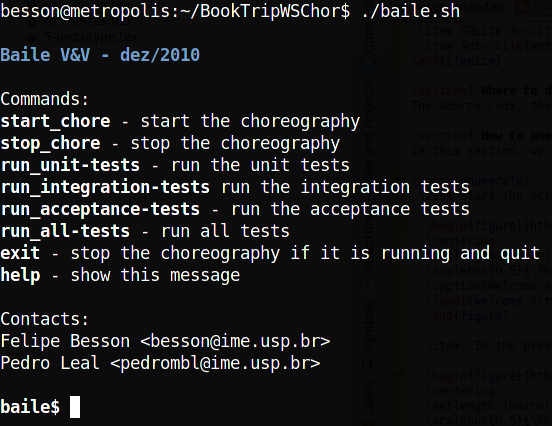
\includegraphics{fig/welcome-screen}}}
  \caption{Welcome screen}
  \label{welcome-screen}
  \end{figure}

  \item  In the prompt, start the coreography by typing \textbf{start\_chore} (as showed in Figure~\ref{chore})
  
  \begin{figure}[htbp]
  \centering
  \setlength\fboxrule{1.0pt}
  \scalebox{0.5}{\fbox{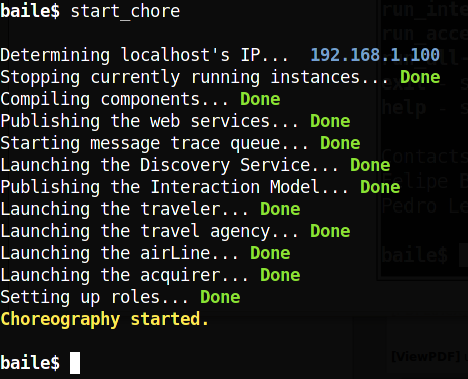
\includegraphics{fig/chore}}}
  \caption{Starting the choreography}
  \label{chore}
  \end{figure}

  \item Once all components of choreography (services, roles, OpenKnowledge entitites) have been started successfully (as showed in Figure~\ref{chore}), the tests can be execute. The following commands are valid:

  \begin{table}[htb]
  \centering
  \begin{tabular}{|l|l|}
  \hline
  Command & Description \\
  \hline
  \hline
  run\_unit-tests & run the unit tests\\
  run\_integration-tests & run the integration tests \\
  run\_acceptance-tests & run the acceptance tests \\
  run\_all-tests & run all tests \\
  \hline
  \end{tabular}
  \end{table}

\end{enumerate}


\section{ How to add more test cases ? }

\section { Project organization }

\section{ Known Issues }

\section{Acknowledgements}
This research received funding from HP Brasil under the Baile Project.

\section{Appendices}


\newpage
\bibliographystyle{abbrv}	% Order by citation
\bibliography{references}

\end{document}

